\documentclass[12pt,a4,english,finnish,pdflatex%,handout
]{beamer}
\definecolor{MyGreen}{RGB}{50, 120, 50}
\usecolortheme[named=MyGreen]{structure}

\usepackage{babel}
\usepackage[utf8]{inputenc}
\usepackage[T1]{fontenc}
\usepackage{amsmath,amssymb} 
\usepackage{animate}
\usepackage{multimedia}

\usepackage{natbib}
\bibpunct[: ]{(}{)}{,}{}{}{;}

\usepackage{tikz}

\usepackage{tipa}

\usepackage{hyperref}

\setbeamertemplate{navigation symbols}{}

\graphicspath{{figures/}}

\setlength{\leftmargini}{0pt}
\setlength{\leftmarginii}{1em}

%% Write out the names of graphics files being included 
\newwrite\graphics
\immediate\openout\graphics=\jobname.graphics%
\let\oincludegraphics\includegraphics% store original \includegraphics
\renewcommand{\includegraphics}[2][]{% prepend to it (could also use xpatch, etc.)
  \immediate\write\graphics{#2}
  \oincludegraphics[#1]{#2}}

\newcommand{\kommentti}[1]{
  {\bf[#1]}
}


\title{Kymography with PATKIT
  \\~\\
  A short introduction to kymography and a promissory note
}
\author{Pertti Palo} 
\date{7 Apr 2025} 


\begin{document}

\frame{\titlepage
  \centering
} 

\frame{\frametitle{Land acknowledgement}
  I would like to respectfully acknowledge that I am today on Treaty 6
  territory in the land now called Canada. My employer -- University of Alberta
  -- is located on land that are traditional homes and gathering places for
  diverse Indigenous peoples including the Cree, Blackfoot, Métis, Nakota
  Sioux, Iroquois, Dene, Ojibway/ Saulteaux/Anishinaabe, Inuit, and many
  others. 
  
  I am a fairly recent uninvited guest in these lands and I have only started
  learning about the histories, languages, and cultures of the local peoples
  and of their historical and continued contribution to our community and how
  to build a better future for all of us. }

\frame{\frametitle{Outline}
  \begin{itemize}
    \item Land acknowledgement
    \item We are here
    \item Who am I?
    \item What is kymography?
    \item Why kymography?
    \item What do we need for kymography?
    \item What is stroboscopy?
    \item What is PATKIT?
    \item The promissory note
    \item MaTiPSS
  \end{itemize}
}

\frame{\frametitle{Who is this Pertti Palo?}
  \begin{columns}
    \begin{column}{5cm}
      \includegraphics[width=\columnwidth]{uti_eva.png}
    \end{column}
    \begin{column}{5cm}
      \begin{itemize}
        \item I have a couple of degrees in engineering and a PhD in Phonetics.
        \item I think of myself as a methods guy and a phonetician.
        \item My life also extends to folk music, folk dancing, oral
        storytelling, wandering (hiking and long distance skiing), role-playing
        games, crafts (knitting, terrain crafting), and other things.
      \end{itemize}
    \end{column}
  \end{columns}
} 

\frame{\frametitle{What is kymography?}
  \begin{itemize}
  \item Kymography -- in general -- is a way of presenting motion or vibration
  as a 2D graph.
  \item Historically this has included such things as waveform traces.
  \item More specifically in the context of laryngoscopy we usually mean
  videokymography which is a technique developed by
  \cite{SvecSchutte-VideokymographyHighspeedLine-1996}.
  \begin{itemize}
    \item Essentially it uses a special camera to capture a line or slice of
    the full view of the camera at an extremely high sample speed and display
    the result as a two-dimensional image where one axis is time.
  \end{itemize} 
  \item Kymography can also refer to any such graph produced from an image
  sequence.
  \end{itemize} 
}

\frame{\frametitle{What is kymography? II}
  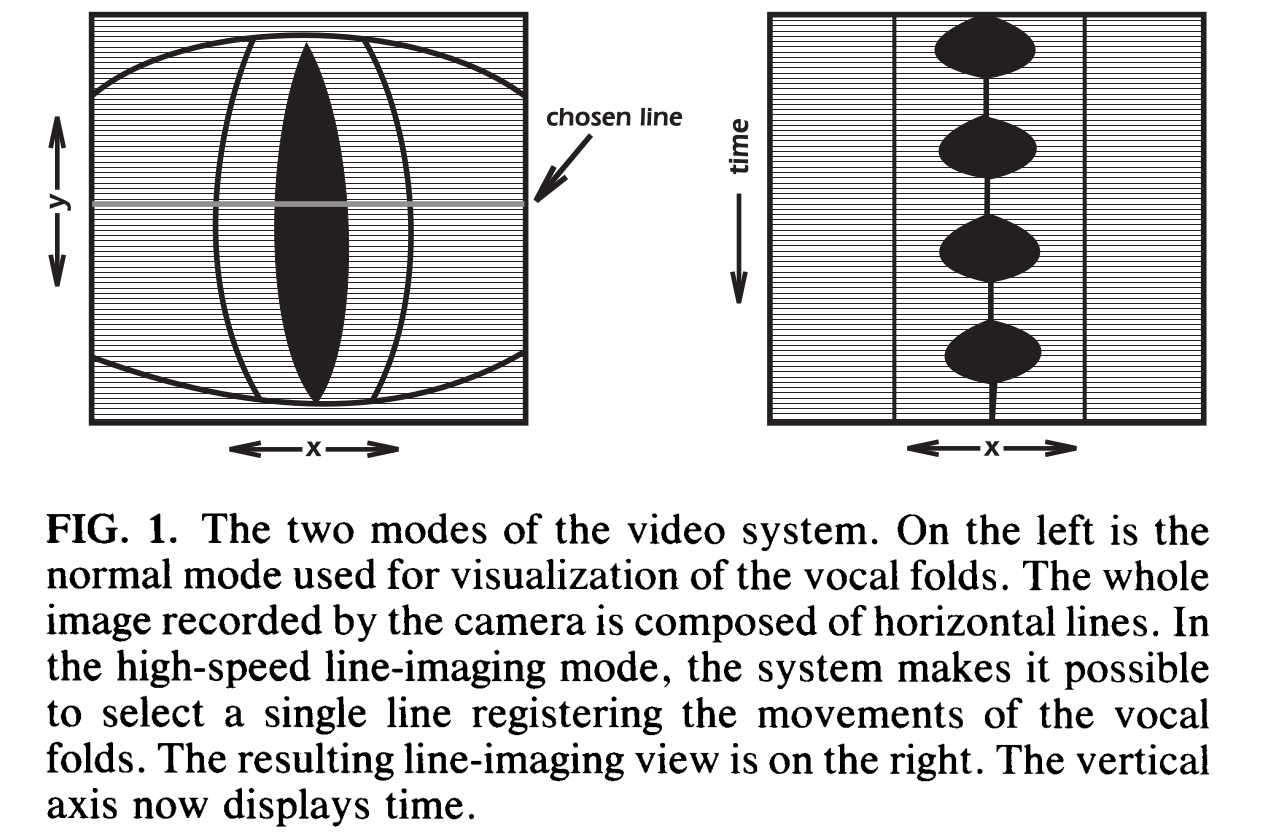
\includegraphics[height=.8\textheight]{kymography_principle_Svec_1996.png}
  Image and caption from \cite{SvecSchutte-VideokymographyHighspeedLine-1996}.
  }

  \frame{\frametitle{What is kymography? III}
  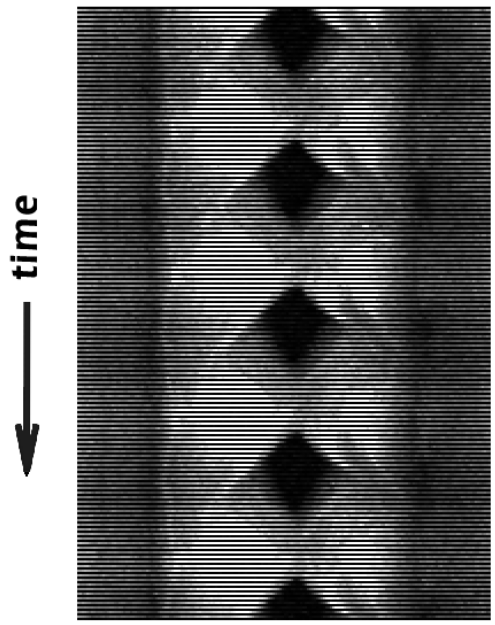
\includegraphics[width=.525\textwidth]{vocal_fold_vibration-Svec-1996.png}
  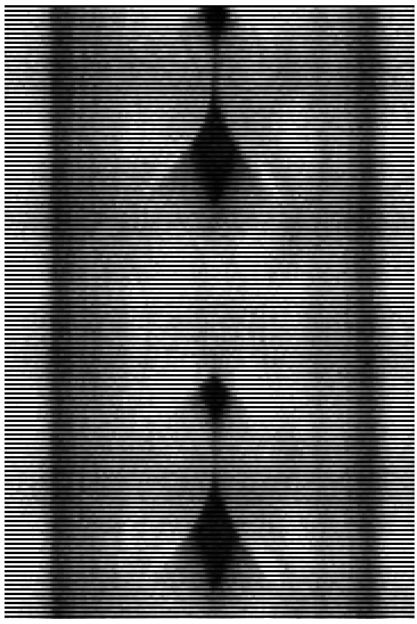
\includegraphics[width=.44\textwidth]{creak-Svec-1996.png}
  Images from \cite{SvecSchutte-VideokymographyHighspeedLine-1996}.
  }

  \frame{\frametitle{Why kymography?}
  \begin{itemize}
    \item If a full frame high speed camera is not available, sampling one line
    at great speeds can be the solution.
    \item Even if a full frame high speed camera is available, kymography can
    provide a handy way of simplifying analysis.
  \end{itemize}
  }
  
  \frame{\frametitle{What do we need for kymography?}
\begin{itemize}
  \item Ideally, high speed -- original was 8000 lines/second -- footage of
  what ever we are studying.
  \item Failing that, just video data of what we are studying.
  \item This can be regular video data. 
  \item For periodic and near periodic phenomena vidoestroboscopy can also be
  an option.  
\end{itemize}
}

\frame{\frametitle{What is stroboscopy?}
\begin{itemize}
  \item Let's have a look at a video \url{https://www.youtube.com/watch?v=g4JBeKvFhz8}
  \citep{WeillCornellSeanParkerInstitutefortheVoice-NormalPhonation-2016}.
  \item Stroboscopy does not work well if e.g. the vocal fold vibration is
  aperiodic, and gives potentially confusing results if the strobe frequency
  and vibration frequency are not matched well. 
\end{itemize}
}

\frame{\frametitle{What is PATKIT?}
\hspace*{-1cm}
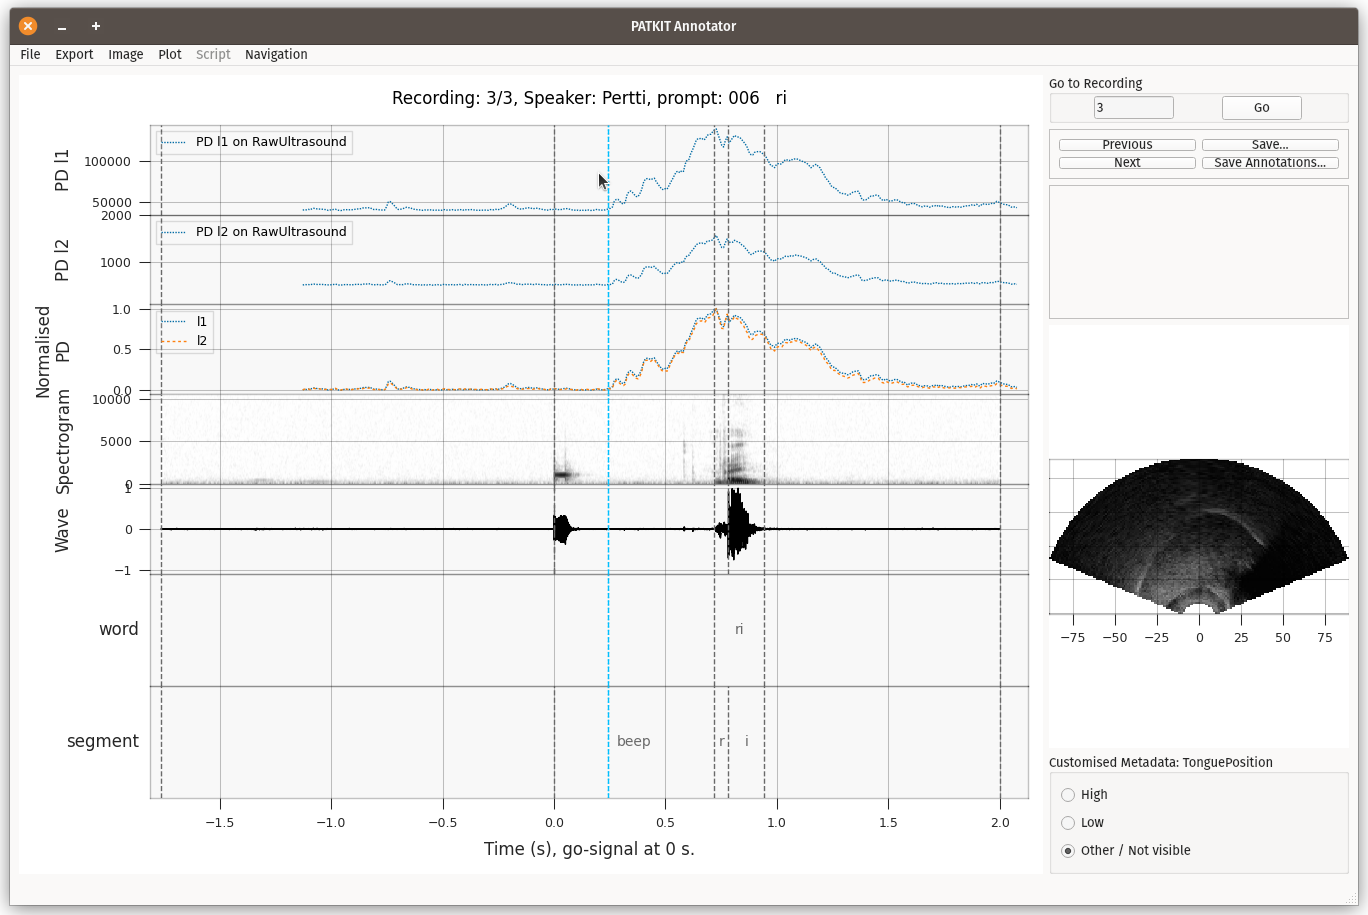
\includegraphics[height=.87\textheight]{patkit_light_mode.png}
}

\frame{\frametitle{The promissory note}
\begin{itemize}
  \item PATKIT \citep{PaloEtAl-PATKITPhoneticAnalysis-2025} \textbf{will} in
  the near future include at least a rudimentary kymograph on arbitrary video
  data.
  \item Concept design and likely tools got selected, if I'd had another half
  day to work on this it would most likely be done.
  \item The caveat is that PATKIT does not magically transform low frame rate
  or stroboscopic data to high frame rate line scanning data.
\end{itemize}
}

\frame{\frametitle{MaTiPSS}
{
  \usebeamercolor[fg]{title}
  Methods and Techniques in Phonetics of Signing and Speech
  }
  \vfill
  \begin{itemize}
    \item Conference concentrating on methodology of signing and speech (with
    broad definitions).
    \item 17-18 October 2025
    \item University of Alberta, Edmonton, Canada
    \item Call for Abstracts will be published soon on Fonetiks newsletter and
    LinguistList.
    \item Ask me for more info.
  \end{itemize}
  }

\frame{
  \centering
  {
    \bf \Large 
    \usebeamercolor[fg]{title}
    Thank you!
    
    \vfill
    For historical reference, as an example of how details matter, and because
    of the wacky title: \cite{Kwan-NotKillGuinea-2016} } }

\frame{\frametitle{References}
  
\bibliographystyle{apalike}
\bibliography{main}

}



\end{document}

